\newprob{1715666204}
{
    % active phys p154(138) q14
    迪生利用圖中的裝置來量度某單色光的波長。光 柵間距為每毫米400條線,其後1 m 置有一塊屏 幕。在屏幕上,兩道第2級亮紋相距1 m。
    \par{\par\centering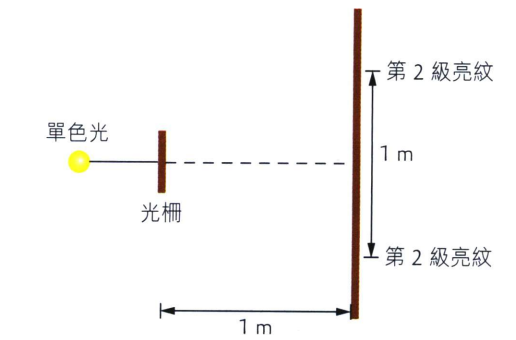
\includegraphics[width=.4\textwidth]{./img/ch4_earlyclass_wave_lq_2024-05-14-14-06-10.png}\par}
    \begin{parts}
        \part 在屏幕上,第2級亮紋與中央最大值之間的 角度為多少?\zzh{2}
        \part 求單色光的波長。\zzh{2}
    \end{parts}
}{
    \sol\par{\par\centering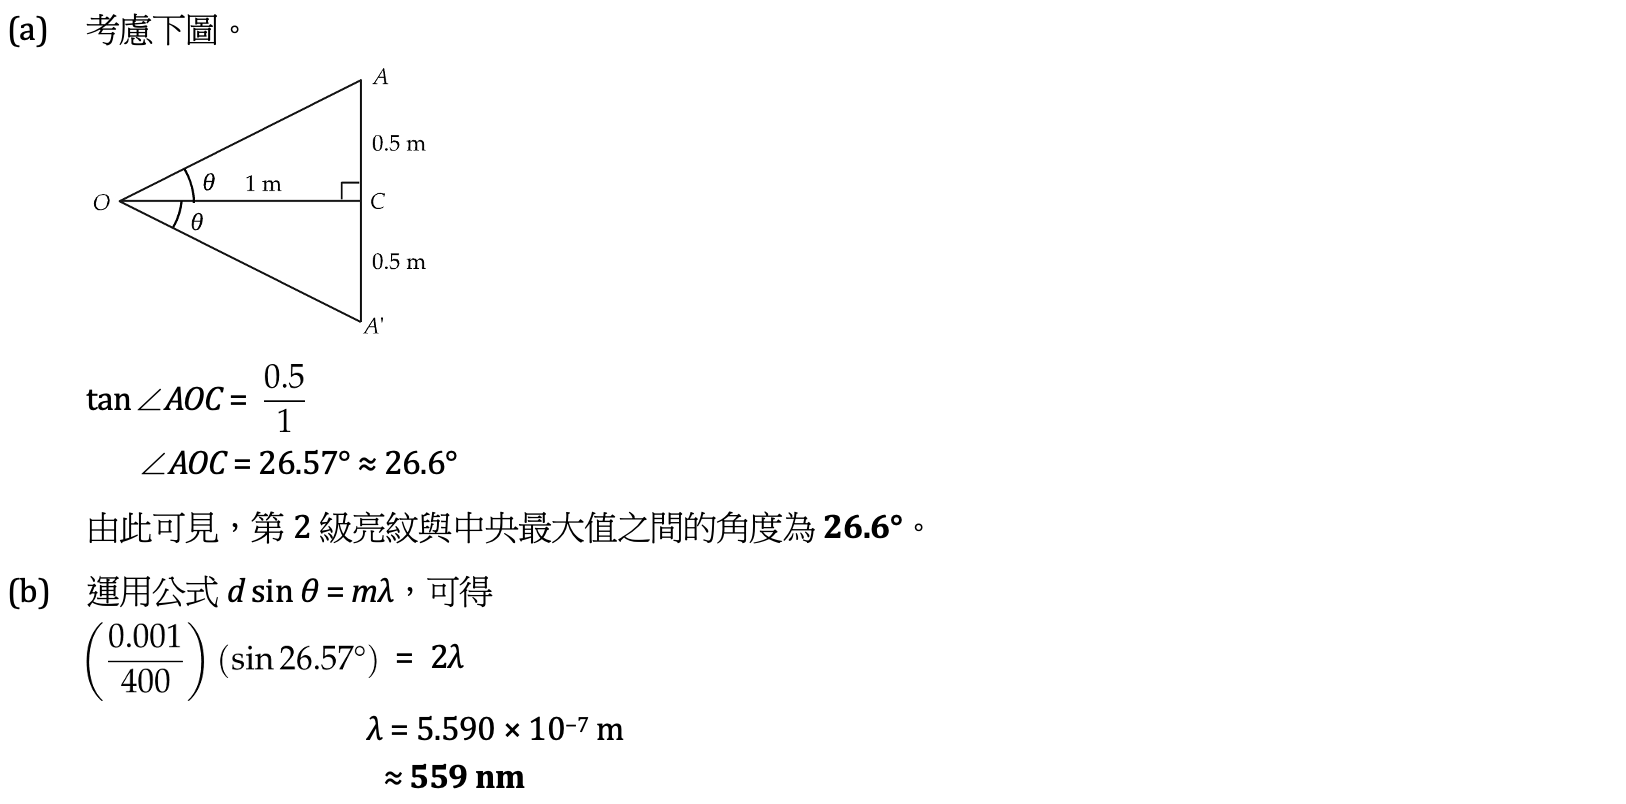
\includegraphics[width=\textwidth]{./img/ch4_earlyclass_wave_lq_2024-05-14-14-07-38.png}\par}
}
\newprob{1715666861}
{
    % active phys p176(160) 17
    在一個雙縫實驗中,明施利用單色光源,在屏幕 上捕捉到干涉圖案,如圖所示。已知雙縫間距為 \qty{20}{\mu m} ,屏幕與雙縫之間的距離為2 m。
    \par{\par\centering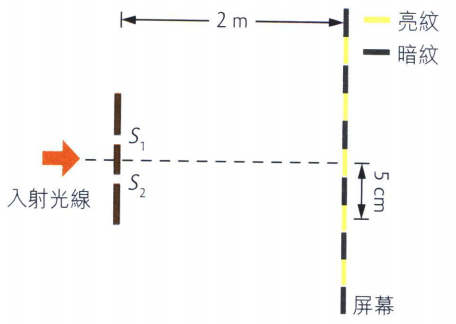
\includegraphics[width=.4\textwidth]{./img/ch4_earlyclass_wave_lq_2024-05-14-14-14-14.png}\par}
    \begin{parts}
        \part 試扼要解釋屏幕上的亮紋與暗紋如何形成。\zzh{2}
        \part 根據以上資料,估計光源放出的單色光的波 長。
        \part 栢豪認為下列措施會增加屏幕上干涉亮紋的 間距。
        \begin{subparts}
            \subpart 使用另一個間距為 \qty{80}{\mu m} 的雙縫
            \subpart 將屏幕移近雙縫
        \end{subparts}
        試評論他的看法。\zzh{2}
    \end{parts}
}{
    \sol\par{\par\centering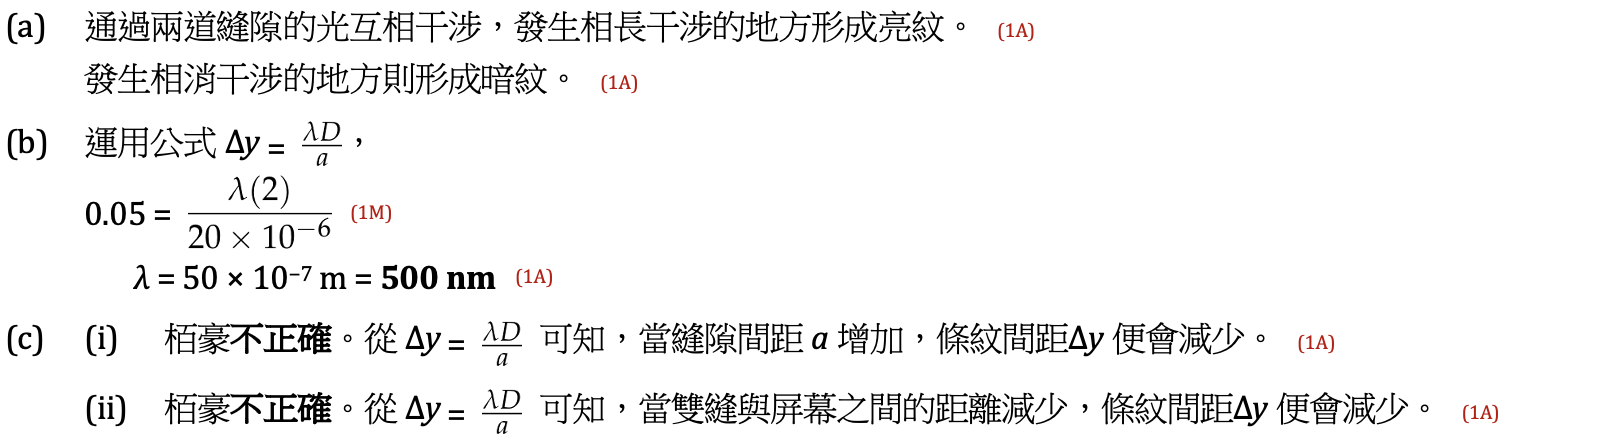
\includegraphics[width=\textwidth]{./img/ch4_earlyclass_wave_lq_2024-05-14-14-16-23.png}\par}
}

\newprob{1715667386}
{
    % active phys p176(160) 18
    現在,你獲得一個單色光源,並有一枝指針、一 塊平面透射光柵(每mm有500線)和兩把米尺。
    \par{\par\centering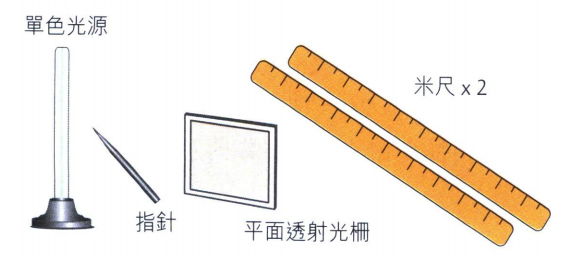
\includegraphics[width=.45\textwidth]{./img/ch4_earlyclass_wave_lq_2024-05-14-14-17-02.png}\par}
    試輔以圖像,說明如何進行實驗來估計該單 色光的波長。\zzh{6}
}{
    \sol \par{\par\centering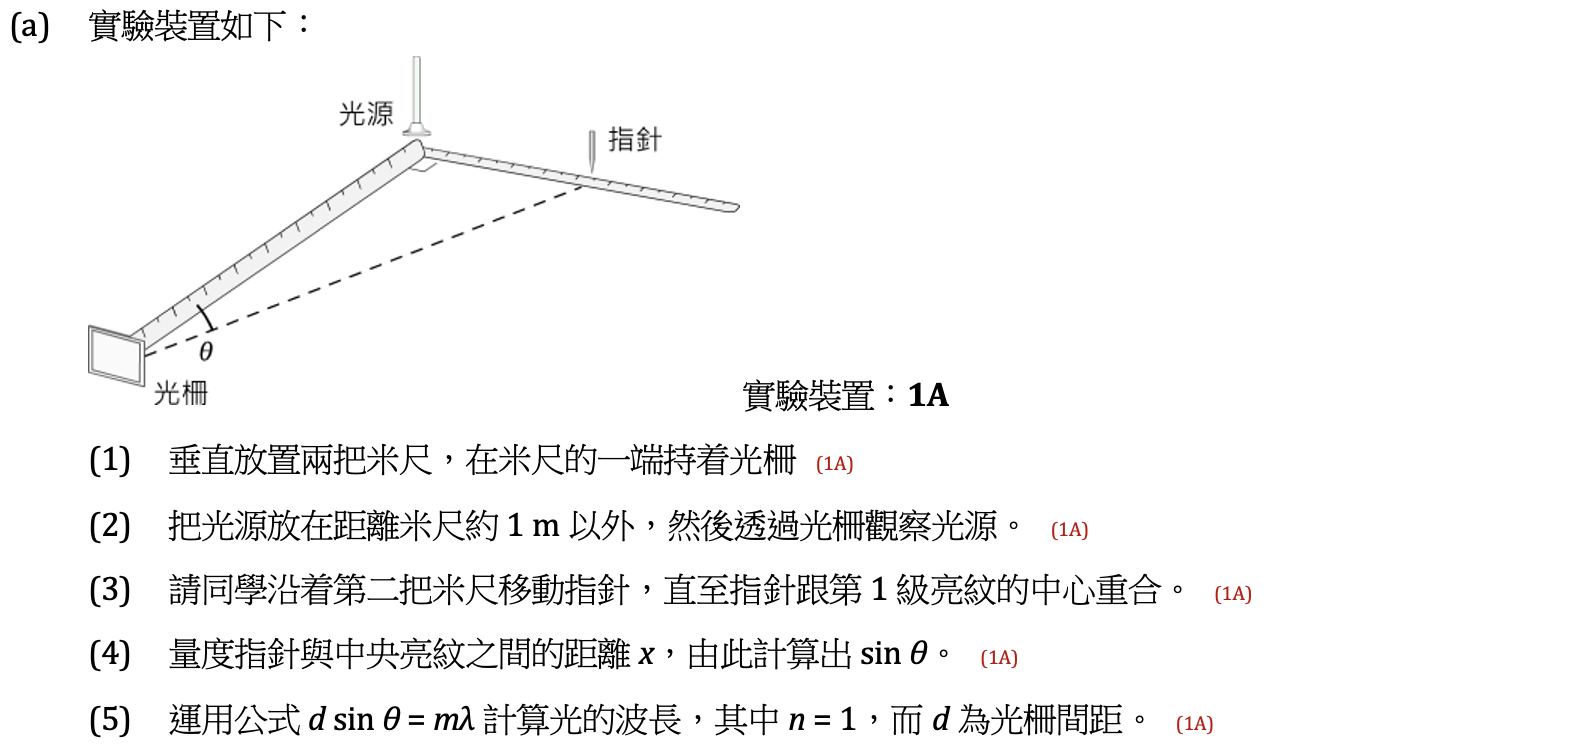
\includegraphics[width=\textwidth]{./img/ch4_earlyclass_wave_lq_2024-05-14-14-18-08.png}\par}
}

\newprob{1715667523}
{
    % q20
    志凡利用下圖所示的光柵光譜儀,觀察一枝鈉光 燈所發射的光譜。在光柵光譜儀上,透射光柵固 定在光譜儀平台上,使鈉光燈發出的光能夠垂直 入射於光柵。
    \par{\par\centering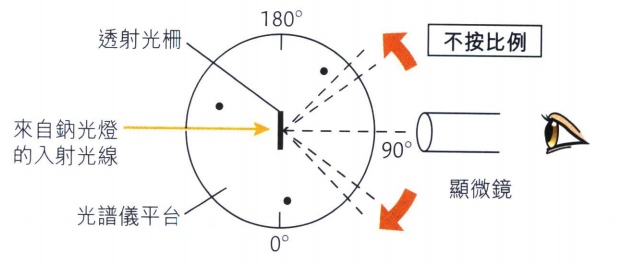
\includegraphics[width=.45\textwidth]{./img/ch4_earlyclass_wave_lq_2024-05-14-14-19-01.png}\par}
    已知鈉光燈所發射的光譜包含兩種波長稍有差別 的黃色色光。志凡以顯微鏡圍繞光譜儀平台,從 中央亮紋起量度兩種色光的第2級亮紋的繞射 角。下表列出相關亮紋的角位置讀數。
    % \par{\par\centering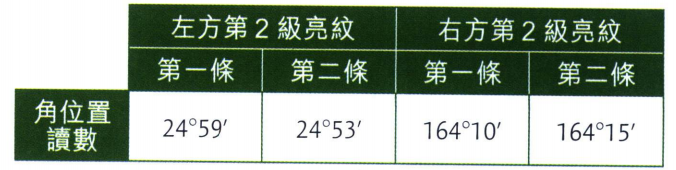
\includegraphics[width=.6\textwidth]{./img/ch4_earlyclass_wave_lq_2024-05-14-14-19-19.png}\par}
    \par{\par\centering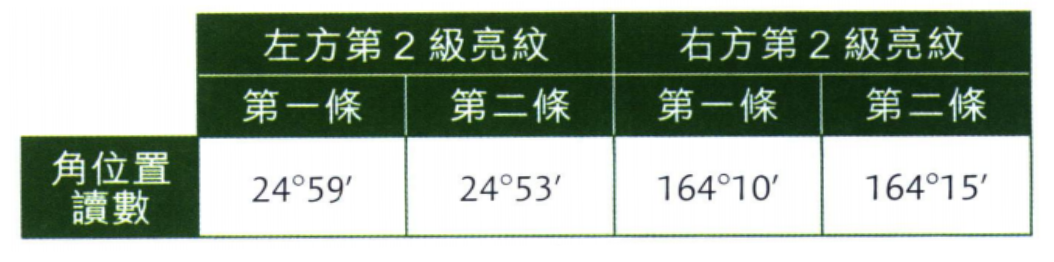
\includegraphics[width=.6\textwidth]{./img/ch4_earlyclass_wave_lq_2024-05-14-14-22-31.png}\par}
    \begin{parts}
        \part 已知透射光柵的光柵間距為 \qty{1256}{nm}。計算 鈉光燈所發射的兩種黃色色光的波長。 (註:\dg{1} $=60'$) \par\zzh{6}
        \part 舉出一個原因,解釋志凡量度繞射亮紋的角 位置時,為何選擇第2級亮紋而不是第1級 亮紋。\zzh{1}
    \end{parts}
}{
    \sol\par{\par\centering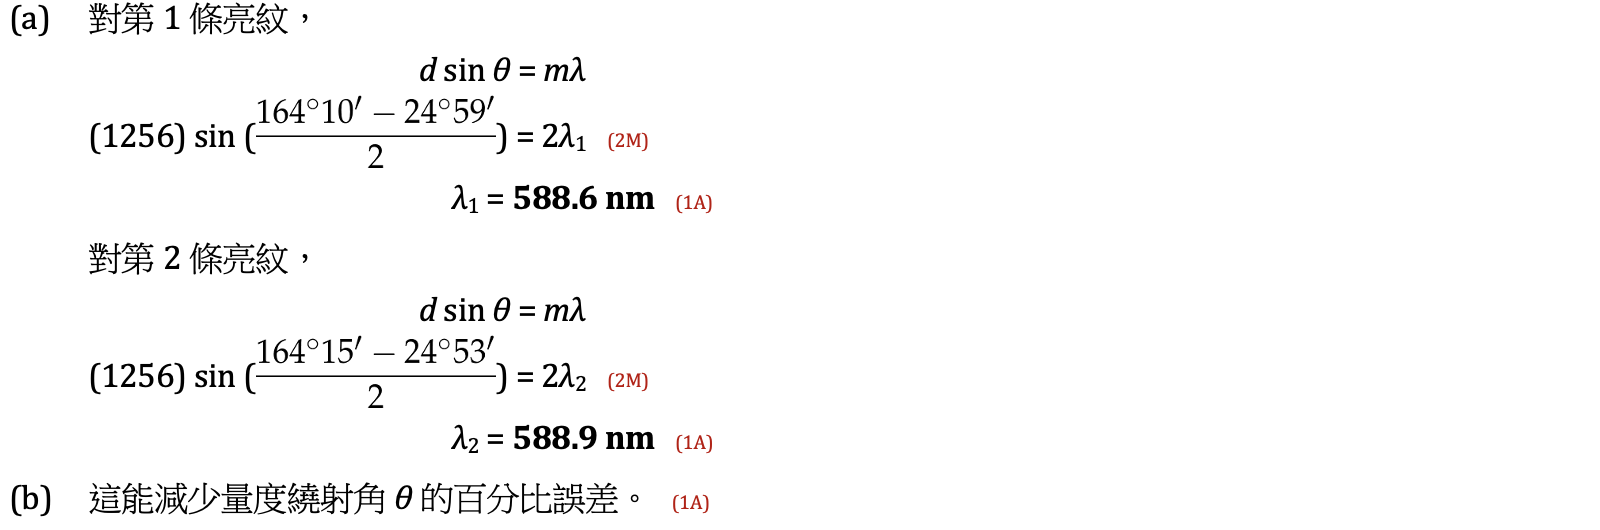
\includegraphics[width=\textwidth]{./img/ch4_earlyclass_wave_lq_2024-05-14-14-24-55.png}\par}
}

\newprob{1715667898}
{
    兩個完全相同的揚聲器$P$和$Q$連接至一個訊號產 生器。位置$O$為$PQ$的中點。振杰沿圖中的直線 $BC$ 移動一個微音器,微音器連接至示波器,用來 量度聲音的強弱變化。
    % \par{\par\centering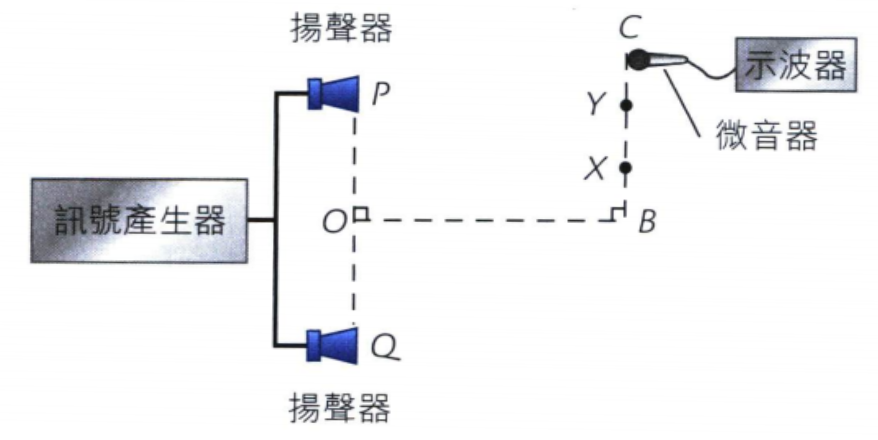
\includegraphics[width=.45\textwidth]{./img/ch4_earlyclass_wave_lq_2024-05-14-14-26-04.png}\par}
    \par{\par\centering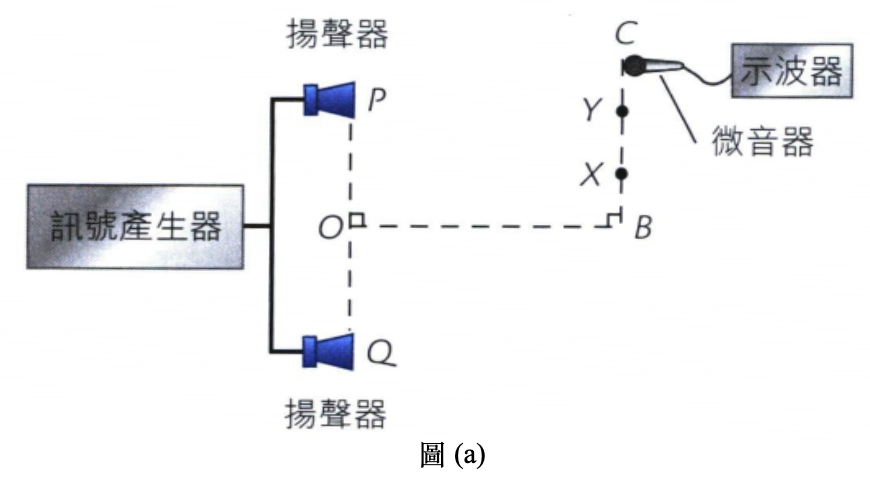
\includegraphics[width=.45\textwidth]{./img/ch4_earlyclass_wave_lq_2024-05-14-14-26-52.png}\par}
    圖b顯示示波器描跡的振幅$A$ 沿直線$BC$的變化。
    \par{\par\centering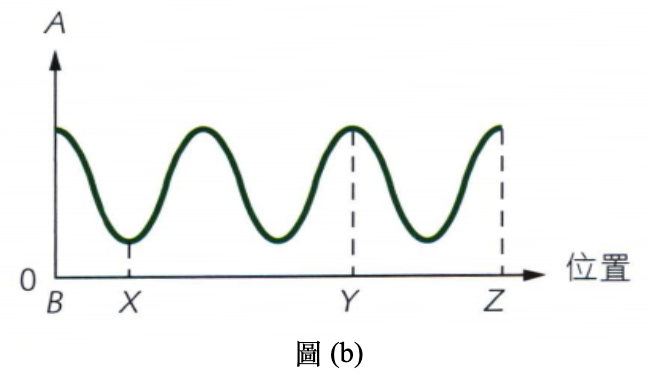
\includegraphics[width=.45\textwidth]{./img/ch4_earlyclass_wave_lq_2024-05-14-14-28-04.png}\par}
    \begin{parts}
        \part
        \begin{subparts}
            \subpart 在直線$BC$上不同的位置,聲音的强弱 不盡相同,試扼要解釋。\zzh{2}
            \subpart 在$X$點,為甚麼示波器描跡的振幅不是 零?\zzh{1}
        \end{subparts}
        \part 已知 $PY= \qty{5.10}{m}$ 和 $QY = \qty{5.78}{m} $。求聲波的 頻率$f_0$。\zzh{3}
        \part 訊號產生器交替發出頻率為$f_0$和$f$的聲波, 其中$f=2f_0$振杰認為在 $Z$ 點將會交替發生 相長和相消干涉。你同意嗎?試加以解釋。\zzh{3}
    \end{parts}
}{\sol\par{\par\centering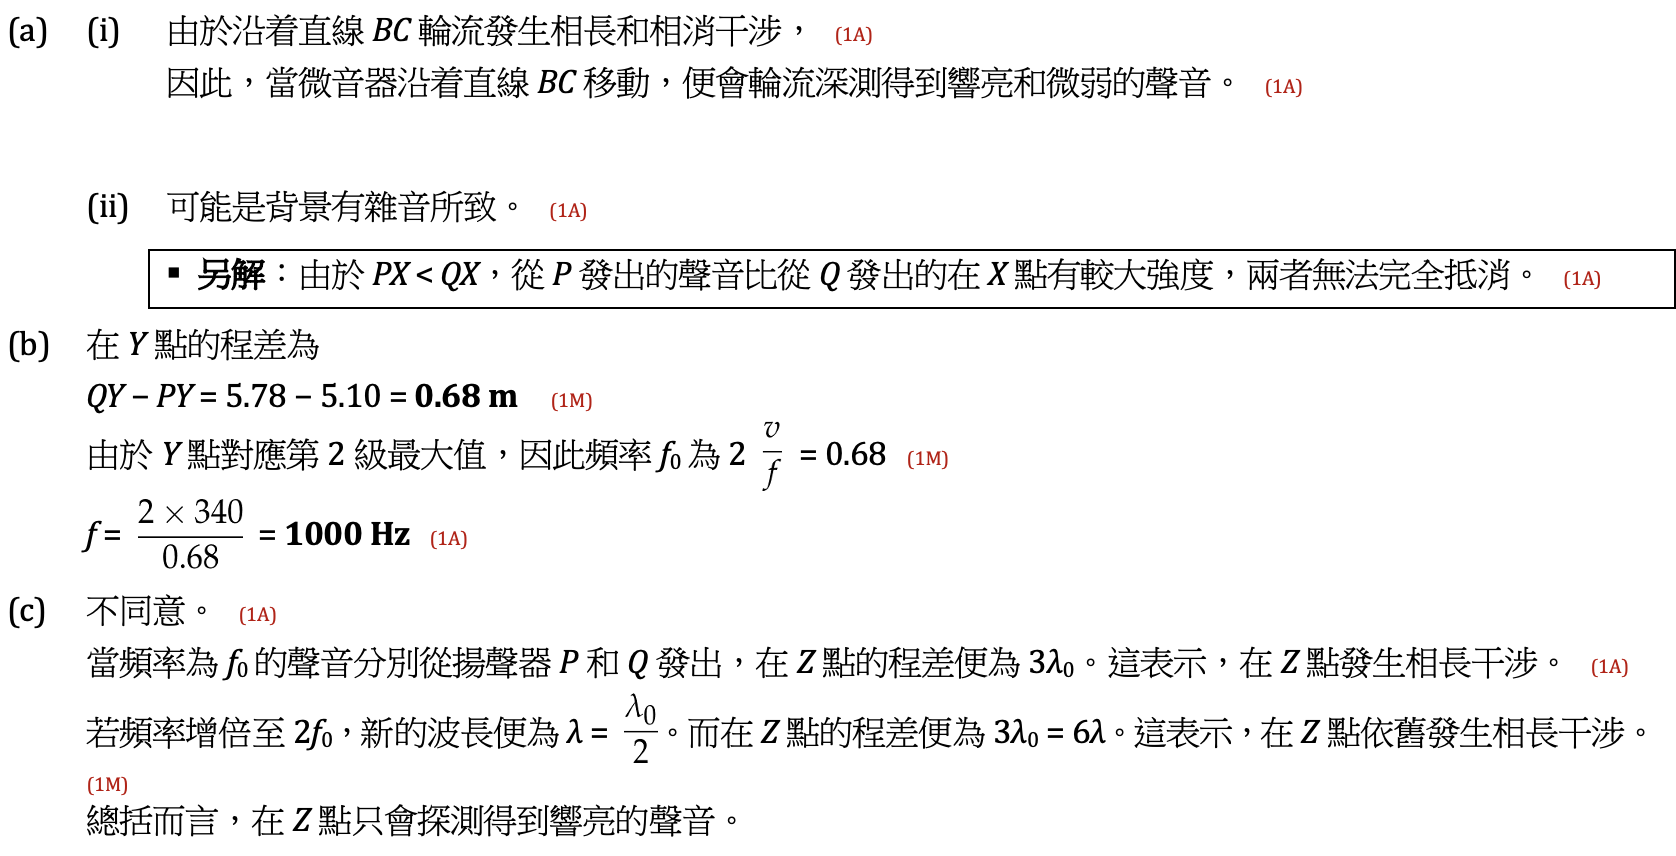
\includegraphics[width=\textwidth]{./img/ch4_earlyclass_wave_lq_2024-05-14-14-32-10.png}\par}}